\documentclass[9pt,twocolumn,letterpaper]{extarticle}
\usepackage[T1]{fontenc}
\usepackage[utf8]{inputenc}
\usepackage{mathptmx}
\usepackage[margin=0.75in,columnsep=0.33in]{geometry}
\usepackage{graphicx}
\usepackage{amsmath}
\usepackage{booktabs}
\usepackage[font=small,labelfont=bf,labelsep=colon]{caption}
\usepackage[compact]{titlesec}
\usepackage{enumitem}
\usepackage{microtype}
\usepackage[hidelinks]{hyperref}
\urlstyle{same}
\usepackage{textcomp}
\usepackage{placeins}

\titleformat{\section}{\normalfont\bfseries\MakeUppercase}{\thesection.}{0.5em}{}
\titleformat{\subsection}{\normalfont\bfseries}{\thesubsection}{0.5em}{}
\titlespacing*{\section}{0pt}{1.1ex plus .3ex}{0.6ex}
\titlespacing*{\subsection}{0pt}{0.9ex plus .2ex}{0.4ex}
\setlist{nosep,leftmargin=1.2em}
\setlength{\textfloatsep}{8pt plus 2pt}
\setlength{\floatsep}{6pt plus 2pt}
\setlength{\abovecaptionskip}{3pt}
\setlength{\belowcaptionskip}{0pt}
\renewcommand{\abstractname}{\normalsize ABSTRACT}

\title{\vspace{-1.5em}\Large\bfseries Missile Strikes, Weather and Rolling Blackouts:\\ A Data-Driven Analysis of Planned Power Outages in Ukraine, 2023--2026}
\author{Danylo Krainii\\[2pt]\normalsize Independent researcher\\\normalsize Student, Lviv Polytechnic National University\\\normalsize Lviv, Ukraine}
\date{}

\begin{document}
\twocolumn[
\maketitle
\vspace{-1.5em}
]

\section*{ABSTRACT}
Since October 2022 Russian missile and drone strikes on Ukraine's power system have forced the transmission system operator to introduce planned stabilisation outages for households. This paper asks which factors determine when such outages are applied. We combine three open datasets into a single hourly panel of 30\,644 hours from January 2023 to June 2026: nationwide outage records of NPC Ukrenergo, weather reanalysis data and a register of 76 massive strikes on energy infrastructure. We show that a recent massive attack is a precondition for outages but not a sufficient condition. Without an attack in the previous 30 days, outages occurred on 2\% of days, compared with 37\% of days after attacks, and they never occurred later than 60 days after an attack. After attacks the share of outage hours follows temperature: 60\% of hours below $-5$\,\textdegree C, 50\% above 25\,\textdegree C and 17\% between 5 and 15\,\textdegree C. These averages hide opposite seasons: cold days after attacks had no outages in early 2025 and round-the-clock outages in early 2026. Weather therefore amplifies outages in seasons when the system is short of capacity, but it does not decide whether attacks lead to outages. A logistic regression with weather--attack interactions ranks hours by risk with a ROC AUC of 0.83 on the unseen 2025/26 season and 0.86 on average in leave-one-wave-out validation, against 0.81 and 0.83 for a baseline that uses attack history only. Its absolute probabilities do not transfer between seasons. After controlling for temperature and attacks, stronger solar radiation is associated with lower odds of an outage, also when radiation is measured against its norm for the month and hour, which is consistent with a contribution of distributed solar generation. Code is open-sourced and all data are publicly available.

\section{Introduction}
Ukraine's electricity system has been a deliberate military target since the full-scale invasion. Strikes intensified in October 2022, brought the grid close to collapse in the winter of 2022/23 and focused on substations and large transformers that are hard to replace~\cite{crs}. A second large wave in spring 2024 destroyed a substantial part of thermal and hydro generation, and the International Energy Agency described the following winter as the sternest test of the system so far~\cite{iea}. To keep the system balanced when demand exceeds available supply, NPC Ukrenergo applies \emph{stabilisation outages}: households are divided into queues that are disconnected in turn according to published hourly schedules.

For households and businesses, these outages are a planning problem. A bakery, a pharmacy or an IT office has to decide when to run a generator, when to schedule work that needs power and how much backup capacity to buy. Public discussion usually explains outages either by attacks or by cold weather, but the relative role of each factor and how they interact have rarely been quantified with open data.

This paper makes the following contributions:
\begin{itemize}
\item an hourly dataset that joins nationwide outage records, weather and the history of massive strikes, with a documented cleaning procedure for data quality problems in the source files, including a time-zone mismatch between the sources;
\item a statistical analysis showing that attacks are a precondition but not a sufficient condition for outages, and that the same weather after attacks led to opposite outcomes in different seasons;
\item an interpretable probabilistic model, validated on an unseen season and across four periods, with an account of what transfers between seasons, the ranking of hours, and what does not, the level of probabilities;
\item estimates of the effects of temperature, attacks and solar radiation in natural units with block-bootstrap intervals, and hour-by-hour scenarios that show how the risk is distributed over the day.
\end{itemize}

The paper is organised as follows. Section~2 reviews related work. Section~3 describes the data and the cleaning procedure. Section~4 presents the exploratory analysis and Section~5 the statistical tests. Section~6 introduces the models and Section~7 their interpretation and scenarios. Section~8 discusses limitations and Section~9 concludes.

\section{Related Work}
\textbf{Weather and electricity demand.} The relationship between air temperature and electricity load is well known to be non-linear. Demand grows both in cold weather because of heating and in hot weather because of cooling, which produces a U-shaped or V-shaped curve with a comfort zone in between~\cite{valor,sailor}. We use the same idea to build piecewise temperature features.

\textbf{Statistical prediction of power outages.} A large body of work predicts outages caused by natural hazards, especially hurricanes, from weather variables and characteristics of the grid~\cite{han,nateghi}. These studies compare generalised linear models with tree-based ensembles and often find that simpler models generalise better to new events. Our setting is different because the main shock is a military attack rather than a storm, but the modelling question is similar.

\textbf{Attacks on Ukraine's power system.} Policy reports by the IEA~\cite{iea} and the U.S.\ Congressional Research Service~\cite{crs} describe the scale of damage, the role of imports from the European grid and the resilience measures taken by Ukraine. To the best of our knowledge, they do not provide an hourly quantitative model that links attacks, weather and outages. This paper aims to fill this gap with open data.

\section{Data}

\subsection{Sources}
Table~\ref{tab:data} lists the three sources. The outage and strike datasets are published by the Energy Map platform of DiXi Group~\cite{dixiout,dixistr}, and the weather data come from the Open-Meteo historical API~\cite{openmeteo}, which is based on the ERA5 reanalysis~\cite{era5}.

\begin{table}[t]
\centering\small
\caption{Data sources. All series end on 30 June 2026.}
\label{tab:data}
\begin{tabular}{@{}p{2.15cm}p{1.15cm}p{3.6cm}@{}}
\toprule
Dataset & Step & Content \\
\midrule
Stabilisation outages~\cite{dixiout} & hour & whether nationwide outages were applied; number of queues; regions; 01.2023--06.2026 \\
Massive strikes~\cite{dixistr} & event & missiles and drones fired and shot down by type; 76 attacks, 09.2022--06.2026 \\
Weather~\cite{openmeteo} & hour & temperature, cloud cover, shortwave radiation, wind speed for Kyiv \\
\bottomrule
\end{tabular}
\end{table}

The outage dataset records only large-scale outages that were applied in all or most regions; local outages in one to three regions are excluded. The strike register likewise contains only attacks officially described as massive by the Ministry of Energy or Ukrenergo, supplemented with Air Force data on the number of weapons; daily local strikes on frontline regions are excluded. Since the outage data are national, we use the weather in Kyiv as a proxy for the whole country.

The same platform publishes hourly cross-border electricity trade~\cite{dixitrade}. It is explored as context in the accompanying notebook but is not used in this paper, because imports respond to the same deficit as outages and cannot serve as an explanatory factor.

\subsection{Cleaning}
Three problems were found in the outage file. First, 328 rows from 1 April 00:00 to 14 April 15:00, 2026 contained spreadsheet formulas instead of the date and hour. Because the order of rows was preserved, the timestamps were restored by adding one hour to the last valid timestamp for each consecutive row. Second, the hour 03:00--04:00 on the last Sunday of October appears twice because of the switch to winter time; the duplicates had identical values and were removed. Third, according to a note by the data provider, hours between 10 December 2025 and 28 January 2026 were aggregated from distribution system operators and do not reflect the real hourly profile. These 1\,200 hours are kept for monthly statistics but excluded from all hourly analysis and modelling, which leaves 29\,444 hours.

A fourth problem concerns the weather file. The API returned the series with a fixed UTC+2 offset, without daylight saving time, while the outage records use Kyiv wall-clock time, which is UTC+3 from late March to late October. Without a correction the weather would be shifted by one hour in 55\% of hours. We convert the weather timestamps to Kyiv time, after which both sources share the same hourly grid. The weather series has no gaps.

\subsection{Attack features}
Massive attacks usually happen at night, while their consequences last for weeks. For each day $d$ we therefore compute features that describe the recent history of attacks. Let $A$ be the set of attack days and $f_t$ the number of missiles and drones fired on day $t$. Then
\begin{align}
\text{days\_since}(d) &= d - \max\{t \in A : t \le d\},\\
\text{attacks}_{30}(d) &= \left|\{t \in A : d-29 \le t \le d\}\right|,\\
\text{fired}_{30}(d) &= \textstyle\sum_{t=d-29}^{d} f_t .
\end{align}
We also compute $\text{attacks}_7$ and the number of weapons that were not shot down within 30 days, an upper-bound proxy for hits. Because the register starts in September 2022, the 30-day history is available from the first day of the study period. The register gives no time of day, so an attack is assigned to its calendar day and the features are the same for all 24 hours of that day, including the hours before the strike. This concerns 56 attack days, 4.6\% of hours.

\section{Exploratory Analysis}

\subsection{When outages happened}
Outages occurred in 16.7\% of the 29\,444 hours used for analysis. Figure~\ref{fig:timeline} shows four episodes: January--February 2023, the end of the winter 2022/23 wave that began before our data start; May--September 2024; November--December 2024; and October 2025--April 2026. In the most severe periods outages were applied in every hour of the day; the longest such period lasted 113 days, from 9 November 2025 to 1 March 2026. The figure also shows that the number of weapons per attack grew several times in 2025--2026.

\begin{figure*}[t]
\centering
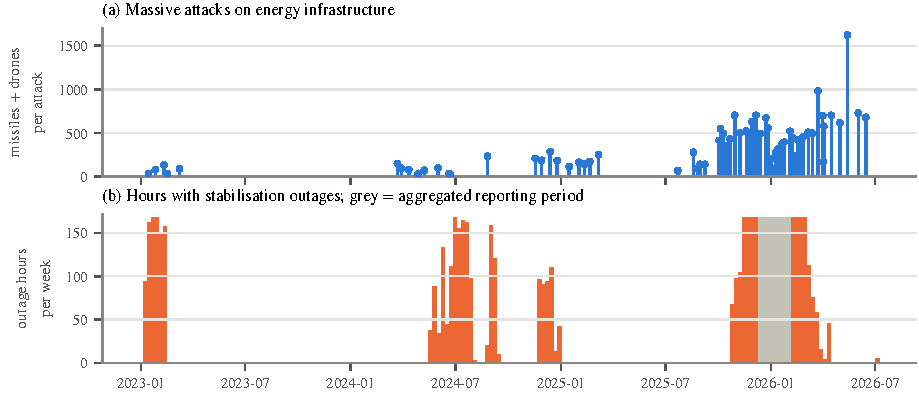
\includegraphics[width=\textwidth]{figures/fig1_timeline.pdf}
\caption{(a) Every massive attack on energy infrastructure and the number of missiles and drones used. (b) Weekly number of hours with nationwide stabilisation outages. Outages follow attacks, but several series of attacks in 2025 and spring 2026 caused no outages.}
\label{fig:timeline}
\end{figure*}

Figure~\ref{fig:heatmap} shows the daily profile by month. Of the 264 days with outages, 143 were round-the-clock days, and they contain 70\% of all outage hours. On such days the hour of day carries no information, so the profile over all days is almost flat: 12.6\% of hours at night against about 20\% in the evening. The daily pattern is visible on the 121 days with partial outages in Figure~\ref{fig:profile}: about 10\% of hours at night, 60--65\% during the working day and 82--90\% in the evening peak from 16:00 to 21:00, when demand is high and solar plants no longer produce. The hourly target therefore mostly reflects differences between days and seasons, not between hours of one day. This matters for the interpretation of the models in Section~6.

\begin{figure}[!t]
\centering
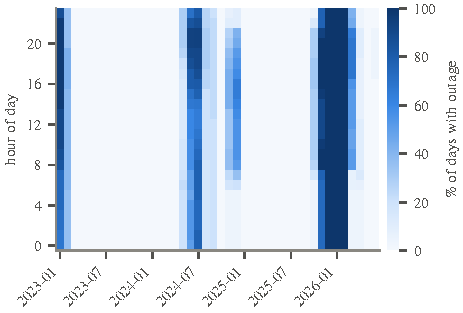
\includegraphics[width=\columnwidth]{figures/fig2_heatmap.pdf}
\caption{Share of days in each month when outages were applied in a given hour. Solid columns correspond to round-the-clock outages. The aggregated period is excluded.}
\label{fig:heatmap}
\end{figure}

\begin{figure}[!t]
\centering
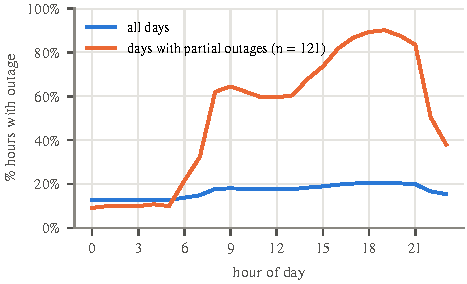
\includegraphics[width=\columnwidth]{figures/fig8_hour_profile.pdf}
\caption{Share of hours with outages by hour of day, for all days and for the days with partial outages, when outages were applied in some but not all 24 hours.}
\label{fig:profile}
\end{figure}

\subsection{Attacks}
Figure~\ref{fig:attacks} shows a strong link between outages and the recent history of attacks. In the first two days after a massive attack, outages were applied in 39\% of hours; after 15--30 days, in 18\%; after 31--60 days, in 3\%; and when more than 60 days had passed, there were no outages at all. The effect accumulates: with no attack in the previous 30 days outages occurred in 0.9\% of hours, and with five or more attacks in 63\%.

All 120 outage hours without an attack in the previous 30 days fall in late July and August 2024, 30 to 60 days after the last attack of that series. In this sample outages thus never occurred later than 60 days after a massive attack. These shares do not measure a recovery time of the system, because the end of a series of attacks usually coincides with a change of season.

\begin{figure}[!t]
\centering
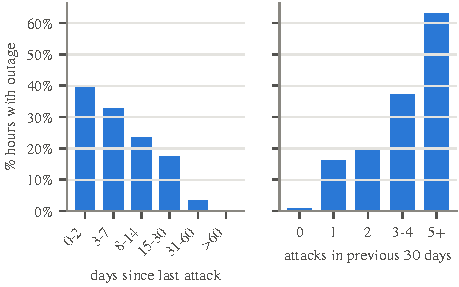
\includegraphics[width=\columnwidth]{figures/fig3_attack_history.pdf}
\caption{Share of hours with outages by days since the last massive attack (left) and by the number of attacks in the previous 30 days (right).}
\label{fig:attacks}
\end{figure}

\subsection{Weather}
The overall relationship with temperature is U-shaped. Between $-20$ and $-15$\,\textdegree C outages were applied in 87\% of hours, between 10 and 15\,\textdegree C in 5.5\%, and between 30 and 35\,\textdegree C again in 37\%. However, cold weather and attacks coincide in time, because the largest attacks take place in winter. Figure~\ref{fig:temp} separates the two factors. Without an attack in the previous 30 days, the share of outage hours was 0\% in all temperature groups up to 15\,\textdegree C and did not exceed 4.6\% even in heat above 25\,\textdegree C. After attacks, the share followed temperature: 60\% of hours below $-5$\,\textdegree C, 50\% above 25\,\textdegree C and 17\% between 5 and 15\,\textdegree C. Section~5 shows that these shares are averages over very different seasons.

\begin{figure}[!t]
\centering
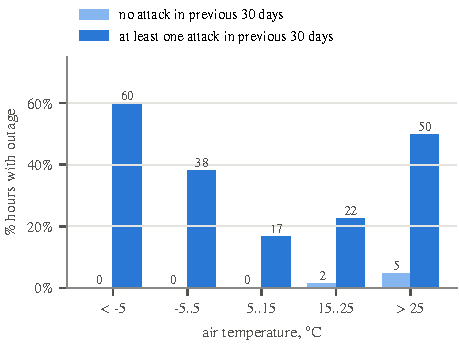
\includegraphics[width=\columnwidth]{figures/fig4_temp_attacks.pdf}
\caption{Share of hours with outages by air temperature, with and without massive attacks in the previous 30 days. Numbers above bars are percentages.}
\label{fig:temp}
\end{figure}

A simple grouping of daytime hours in the warm season by solar radiation showed the opposite of what was expected: more outages on sunnier days. Almost all daytime warm-season outages took place in summer 2024, when sunny days were also the hottest. Radiation is correlated with temperature, so this grouping mixes the two effects. We return to this question with a multivariate model in Section~7.

\section{Statistical Tests}
Neighbouring hours are strongly dependent: if an outage is applied at 18:00, it is almost certainly applied at 19:00 as well. Tests on hourly data would therefore give overly optimistic p-values. We aggregate the data to 1\,227 days and use, for each day, the share of hours with outages. Even daily observations are autocorrelated because outage periods last for weeks, so we report p-values only as a guide and focus on effect sizes. Table~\ref{tab:tests} summarises the results.

\begin{table}[t]
\centering\small
\caption{Hypothesis tests on daily data. Shares are mean shares of outage hours per day unless stated otherwise.}
\label{tab:tests}
\begin{tabular}{@{}p{2.75cm}p{3.05cm}l@{}}
\toprule
Hypothesis & Effect & Supported \\
\midrule
H1: attacks in previous 30 days are associated with outages & days with outages: 2.0\% vs 37.1\%; $\chi^2 = 218.7$, Cram\'er's $V = 0.42$ & yes \\
\addlinespace
H2: risk decreases with time since attack & Spearman $\rho = -0.45$; within 60 days $\rho = -0.29$ & yes \\
\addlinespace
H3a: after attacks, cold days have more outages than mild days & 52.8\% vs 13.3\%; Mann--Whitney $p < 10^{-18}$ & on average \\
\addlinespace
H3b: after attacks, hot days have more outages than mild days & 49.6\% vs 13.3\%; Mann--Whitney $p < 10^{-10}$ & on average \\
\addlinespace
H4: fewer outages on weekends & 25.9\% vs 30.7\%; $p = 0.12$ & no \\
\bottomrule
\end{tabular}
\end{table}

For H1 we use the $\chi^2$ test on a $2\times2$ table of days with and without recent attacks against days with and without outages, and Cram\'er's $V=\sqrt{\chi^2/n}$ as the effect size. For H2 we use Spearman's rank correlation, which requires only a monotone relationship. For H3 and H4 we compare days within the attacked periods using the one-sided Mann--Whitney test~\cite{mann} implemented in SciPy~\cite{scipy}, which does not assume normality. Cold days are days with a mean temperature below 0\,\textdegree C, mild days between 5 and 20\,\textdegree C, and hot days above 22\,\textdegree C.

\textbf{Attacks are not a sufficient condition.} Table~\ref{tab:quarters} shows the same data by quarter. In the first and third quarters of 2025 there were five massive attacks each, but not a single hour of nationwide outages. In the second quarter of 2026 there were eight attacks, the most powerful in the whole period by the number of weapons, and outages were applied in only 2.5\% of hours. Note also that the absolute number of weapons grew more than tenfold between 2023 and 2026, so it cannot be compared directly across years.

\begin{table}[t]
\centering\small
\caption{Attacks and outages by quarter. Fired: mean number of missiles and drones in the previous 30 days.}
\label{tab:quarters}
\begin{tabular}{@{}lrrrr@{}}
\toprule
Quarter & Attacks & Fired & Outage hours & Mean temp. \\
\midrule
2023 Q1 & 5 & 163 & 41.6\% & 1.3\,\textdegree C \\
2023 Q2--Q4 & 0 & $\le 7$ & 0.0\% & 5--21\,\textdegree C \\
2024 Q1 & 2 & 20 & 0.0\% & 1.5\,\textdegree C \\
2024 Q2 & 6 & 166 & 28.2\% & 16.1\,\textdegree C \\
2024 Q3 & 1 & 91 & 40.4\% & 22.0\,\textdegree C \\
2024 Q4 & 4 & 203 & 20.2\% & 4.4\,\textdegree C \\
2025 Q1 & 5 & 352 & 0.0\% & 1.7\,\textdegree C \\
2025 Q2 & 0 & 14 & 0.0\% & 14.7\,\textdegree C \\
2025 Q3 & 5 & 227 & 0.0\% & 19.9\,\textdegree C \\
2025 Q4 & 11 & 1\,898 & 58.8\% & 7.0\,\textdegree C \\
2026 Q1 & 9 & 2\,082 & 69.1\% & $-0.2$\,\textdegree C \\
2026 Q2 & 8 & 2\,132 & 2.5\% & 15.1\,\textdegree C \\
\bottomrule
\end{tabular}
\end{table}

\textbf{Same weather, different seasons.} Mild weather does not explain the quiet quarters: the first quarter of 2025 was as cold as the first quarter of 2023. Table~\ref{tab:seasons} takes the cold and hot days of H3 and splits them by quarter. On cold days after attacks, outages covered 67\% of hours in early 2023, 52\% in late 2024 and 100\% in early 2026, but 0\% in early 2025, although those 33 days were colder on average than the cold days of 2023 and 2024. On hot days after attacks the share was about 90\% in summer 2024 and 0--1\% in 2025 and 2026.

\begin{table}[t]
\centering\small
\caption{Days after attacks with the same weather, by quarter. Cold: mean temperature below 0\,\textdegree C. Hot: above 22\,\textdegree C. The aggregated period is excluded.}
\label{tab:seasons}
\begin{tabular}{@{}llrrr@{}}
\toprule
Days & Quarter & Days & Outage hours & Mean temp. \\
\midrule
Cold & 2023 Q1 & 39 & 67.4\% & $-2.6$\,\textdegree C \\
 & 2024 Q4 & 19 & 52.2\% & $-2.0$\,\textdegree C \\
 & 2025 Q1 & 33 & 0.0\% & $-4.5$\,\textdegree C \\
 & 2026 Q1 & 25 & 100.0\% & $-8.2$\,\textdegree C \\
\addlinespace
Hot & 2024 Q2 & 6 & 87.5\% & 23.5\,\textdegree C \\
 & 2024 Q3 & 30 & 90.8\% & 25.1\,\textdegree C \\
 & 2025 Q3 & 15 & 0.0\% & 23.6\,\textdegree C \\
 & 2026 Q2 & 15 & 1.4\% & 24.1\,\textdegree C \\
\bottomrule
\end{tabular}
\end{table}

The averages of H3 are therefore averages over seasons of two kinds, almost everything or nothing. Weather amplifies outages in a season when the system is short of capacity, but it does not decide whether a series of attacks turns into outages. That depends on the state of the system: what was damaged, how quickly it was repaired and how much could be imported. These factors are not observed in our data. For the same reason the 116 cold days and 66 hot days are not independent observations. Each group comes from four quarters, so the p-values of H3 overstate the strength of the evidence.

\section{Models}

\subsection{Problem statement}
Let $y_h \in \{0,1\}$ indicate whether nationwide outages were applied in hour $h$, and let $\mathbf{x}_h$ be a vector of features. We estimate the probability $p_h = P(y_h = 1 \mid \mathbf{x}_h)$.

Only features that do not depend on the outages themselves are used: hour of day, day of week, weather and the history of attacks. Net import and the number of queues are excluded. Imports grow at the same time as outages in response to the same deficit, and the number of queues is known only once outages have already been applied, so both would leak information about the target. Two reservations apply. The weather is observed weather, not a forecast, and on attack days the attack features are not yet known in the hours before the strike.

\subsection{Logistic regression}
To describe the U-shape found in Section~4, temperature $T_h$ is split into two piecewise linear features,
\begin{equation}
c_h = \max(0,\, 10 - T_h), \qquad w_h = \max(0,\, T_h - 20),
\end{equation}
the number of degrees below 10\,\textdegree C and above 20\,\textdegree C. Because Section~4 showed that weather matters only after attacks, we add interactions with an indicator $r_h = \mathbf{1}[\text{attacks}_{30} > 0]$. The model is
\begin{equation}
\operatorname{logit}(p_h) = \beta_0 + \boldsymbol{\beta}^{\top}\mathbf{z}_h + \gamma_1 c_h r_h + \gamma_2 w_h r_h + \gamma_3 s_h r_h + \alpha_{\text{hour}(h)},
\end{equation}
where $\mathbf{z}_h$ contains $c_h$, $w_h$, solar radiation $s_h$, cloud cover, wind speed, a weekend indicator, $\log(1+\text{days\_since})$, $\text{attacks}_{30}$ and $r_h$, and $\alpha_{\text{hour}}$ are fixed effects for the hour of day. Numeric features are standardised before fitting, and the model is fitted with L2 regularisation in scikit-learn~\cite{sklearn}. For interpretation the coefficients are converted back to natural units in Section~7.

As a baseline we fit a logistic regression with attack history only: $\text{attacks}_{30}$, $\log(1+\text{days\_since})$ and $r_h$. It shows how much weather and hour of day add.

\subsection{Gradient boosting}
As a flexible alternative we use histogram-based gradient boosting of decision trees~\cite{friedman,lightgbm} on the raw features: hour, day of week, temperature, radiation, cloud cover, wind, days since attack, attacks in 7 and 30 days, weapons fired and not shot down in 30 days. Boosting can find non-linearities and interactions on its own. We use 300 trees of depth at most 4, a learning rate of 0.05 and at least 200 samples per leaf to limit overfitting. A second version without the two weapon-count features shows how much boosting depends on them.

\subsection{Validation}
A random split would put neighbouring hours into both training and test sets and overestimate quality. We therefore use two time-aware schemes. In the main scheme, models are trained on 24\,093 hours before 1 October 2025, when outages occurred in 11.8\% of hours, and tested on 5\,351 hours of the 2025/26 season, when they occurred in 38.7\% of hours. In the second scheme, leave-one-wave-out, the data are divided into four periods: W1 January--September 2023, W2 October 2023--September 2024, W3 October 2024--September 2025 and W4 October 2025--June 2026. Each period is predicted by a model trained on the other three. W4 coincides with the main scheme.

We report ROC AUC, the area under the precision--recall curve (PR AUC), the Brier score $\frac{1}{n}\sum_h (p_h - y_h)^2$ and the mean predicted probability, which should be close to the observed share of outages if the model estimates the overall risk correctly.

\subsection{Results}
Table~\ref{tab:metrics} shows that all models rank hours far better than the base rate. Gradient boosting ranks best, with ROC AUC 0.86 against 0.83 for the logistic regression, but it strongly underestimates the risk: its mean predicted probability is 10\% while the observed share is 39\%. Its ranking depends on the numbers of weapons, and without them its ROC AUC falls to 0.64. The baseline with attack history only reaches 0.81. On this season, weather and hour of day therefore add little to the ranking and improve mainly the Brier score, 0.174 against 0.193.

\begin{table}[t]
\centering\small
\caption{Results on the unseen 2025/26 season. Observed share of outage hours: 0.387.}
\label{tab:metrics}
\begin{tabular}{@{}p{2.75cm}rrrr@{}}
\toprule
Model & ROC AUC & PR AUC & Brier & Mean $p$ \\
\midrule
Base rate & 0.500 & 0.387 & 0.309 & 0.118 \\
Attack history only & 0.813 & 0.674 & 0.193 & \textbf{0.381} \\
Logistic regression & 0.826 & 0.680 & \textbf{0.174} & 0.364 \\
Gradient boosting & \textbf{0.862} & \textbf{0.823} & 0.263 & 0.100 \\
Gradient boosting, no weapon counts & 0.636 & 0.454 & 0.291 & 0.223 \\
\bottomrule
\end{tabular}
\end{table}

The mean probability of the logistic regression, 36\%, is close to the observed 39\%, but Table~\ref{tab:calib} shows that this is the result of errors that cancel out. The model underestimates the crisis months, with 37\% predicted against 87\% observed in November 2025 and 64\% against 100\% in February 2026, and overestimates the quiet spring, with 33\% against 7\% in April and 18\% against 0\% in May 2026.

\begin{table}[t]
\centering\small
\caption{Logistic regression on the 2025/26 season by month: observed share of outage hours and mean predicted probability. December and January contain only hours outside the aggregated period.}
\label{tab:calib}
\begin{tabular}{@{}lrrr@{}}
\toprule
Month & Hours & Observed & Predicted \\
\midrule
October 2025 & 744 & 19.5\% & 33.7\% \\
November 2025 & 720 & 87.1\% & 37.5\% \\
December 2025 & 216 & 100.0\% & 47.1\% \\
January 2026 & 72 & 100.0\% & 66.4\% \\
February 2026 & 672 & 100.0\% & 63.7\% \\
March 2026 & 743 & 38.2\% & 36.7\% \\
April 2026 & 720 & 6.9\% & 33.0\% \\
May 2026 & 744 & 0.0\% & 18.3\% \\
June 2026 & 720 & 0.7\% & 27.8\% \\
\bottomrule
\end{tabular}
\end{table}

Table~\ref{tab:cv} gives the leave-one-wave-out results. On average over the four waves the logistic regression ranks best, with AUC 0.86 against 0.83 for boosting and 0.83 for the attack-only baseline; boosting without weapon counts reaches 0.70. Wave W2 is the hardest, because it contains the first summer outages of 2024. On W2 the attack-only baseline is better than both full models, so the weather relationships learned from the other periods did not transfer to that summer.

The level of risk does not transfer between waves either. For W2 the logistic regression predicts a mean probability of 1\% against the observed 17\%, for W3 23\% against 5\%, and in both waves its Brier score is worse than that of the base rate. We use the logistic regression in the rest of the paper because of its better average ranking and its interpretability, and we use it to compare conditions with each other, not to state absolute probabilities.

\begin{table*}[t]
\centering\small
\caption{Leave-one-wave-out validation. ROC AUC of the attack-only baseline, the logistic regression and gradient boosting; mean predicted probability and Brier score of the logistic regression; Brier score of the base rate.}
\label{tab:cv}
\begin{tabular}{@{}lrrrrrrrr@{}}
\toprule
 & & & \multicolumn{3}{c}{ROC AUC} & \multicolumn{2}{c}{Logistic regression} & Base rate \\
\cmidrule(lr){4-6}\cmidrule(lr){7-8}\cmidrule(l){9-9}
Test wave & Hours & Outage share & Attacks only & Logistic & Boosting & Mean $p$ & Brier & Brier \\
\midrule
W1: 01--09.2023 & 6\,551 & 0.137 & 0.939 & 0.956 & \textbf{0.973} & 0.113 & 0.069 & 0.120 \\
W2: 10.2023--09.2024 & 8\,783 & 0.171 & \textbf{0.824} & 0.752 & 0.684 & 0.009 & 0.169 & 0.142 \\
W3: 10.2024--09.2025 & 8\,759 & 0.051 & 0.763 & \textbf{0.896} & 0.786 & 0.230 & 0.107 & 0.076 \\
W4: 10.2025--06.2026 & 5\,351 & 0.387 & 0.813 & 0.826 & \textbf{0.862} & 0.364 & 0.174 & 0.309 \\
\midrule
Mean & & & 0.835 & \textbf{0.857} & 0.826 & & & \\
\bottomrule
\end{tabular}
\end{table*}

\section{Interpretation and Scenarios}

\subsection{Which factors matter}
The logistic regression is refitted on all data. Because of the interactions, the effect of weather after attacks is the sum of a main coefficient and an interaction, and the two should not be read separately. Per standard deviation the interaction of cold with recent attacks has an odds ratio of 13.5 and cold alone 0.09, but the latter is estimated on 5\,187 hours without recent attacks and below 10\,\textdegree C, among which there was not a single outage hour. It only cancels the interaction where there were no attacks.

Figure~\ref{fig:odds} therefore shows odds ratios in natural units and, for weather, for hours after recent attacks. The intervals are 95\% percentile intervals from a block bootstrap in which whole calendar months are resampled and the model is refitted 300 times. Months are used as blocks because outage periods last for weeks.

\begin{figure}[!t]
\centering
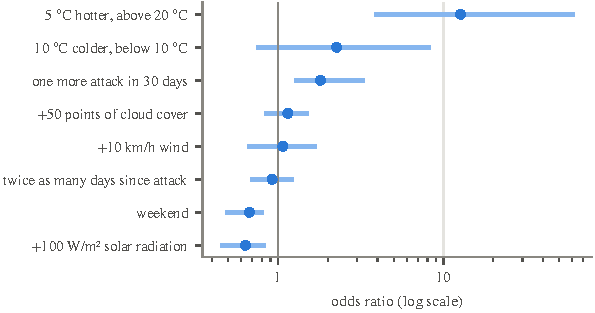
\includegraphics[width=\columnwidth]{figures/fig5_odds.pdf}
\caption{Odds ratios of the logistic regression in natural units with 95\% block-bootstrap intervals. Weather effects are for hours with at least one attack in the previous 30 days. Hour fixed effects are not shown.}
\label{fig:odds}
\end{figure}

Heat has the largest effect: 5\,\textdegree C above 20\,\textdegree C multiply the odds by 12.7, with an interval of 3.8--62. This estimate rests mostly on one summer, 2024. Cold has a smaller and uncertain effect: 10\,\textdegree C below 10\,\textdegree C multiply the odds by 2.3, with an interval of 0.7--8.4 that includes 1, which agrees with Table~\ref{tab:seasons}. Each additional attack in 30 days multiplies the odds by 1.8, interval 1.3--3.3. The weekend odds ratio is 0.67, interval 0.48--0.82, although H4 was not significant on daily data, so the evidence on weekends is mixed. Time since the last attack, cloud cover and wind have intervals that include 1.

Solar radiation is associated with lower odds of an outage: 100\,W/m$^2$ more multiply the odds by 0.64, interval 0.45--0.84. Radiation follows a regular daily and seasonal cycle, so this coefficient may partly reflect the season. As a robustness check we replace radiation by its deviation from the mean for the same month and hour, that is by how sunny the hour was compared with its norm, and drop cloud cover, which measures the same thing. The effect keeps its direction but is less than half as strong: 0.83, interval 0.72--0.95. The hypothesis that distributed solar generation lowers the risk, which could not be confirmed by the simple grouping in Section~4, is consistent with the data. It is not proven, because the actual output of solar plants is not observed.

The intervals should be read as approximate. The main variation is between seasons, and there are few seasons with outages, so even month blocks may understate the uncertainty.

To measure the importance of groups of features we use permutation importance~\cite{breiman}: the values of a group are shuffled in the test set, derived features are recomputed, and the decrease in ROC AUC is recorded. The history of attacks is the most important group, with a decrease of 0.176, followed by solar radiation and cloud cover with 0.143 and hour of day with 0.071. Temperature has a small importance of 0.027 in this test because the 2025/26 season was almost entirely cold, so shuffling temperature within it changes little. Weekend and wind are not important.

\subsection{Partial dependence}
Figure~\ref{fig:pdp} shows partial dependence plots~\cite{friedman}, the average predicted probability when one feature is varied and the others keep their observed values, for hours with at least one attack in the previous 30 days. The risk is lowest at 18\% between 10 and 20\,\textdegree C, rises gradually with frost to 52\% at $-15$\,\textdegree C and sharply above 22\,\textdegree C. Values above 30\,\textdegree C should be interpreted with caution because such hours are rare and belong almost entirely to one summer. Stronger solar radiation lowers the average risk from 40\% without sun to 4\% at 850\,W/m$^2$. Both curves are averages over seasons with very different outcomes. They show the direction and shape of the relationships, not the level to expect in a particular season.

\begin{figure}[!t]
\centering
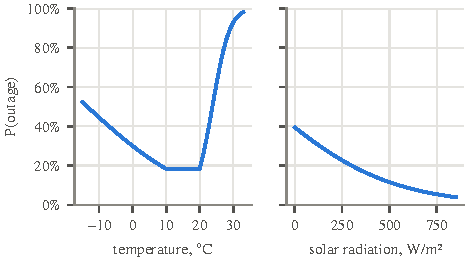
\includegraphics[width=\columnwidth]{figures/fig6_pdp.pdf}
\caption{Partial dependence of the outage probability on temperature and solar radiation. Computed with the logistic regression on 4\,000 hours with at least one attack in the previous 30 days.}
\label{fig:pdp}
\end{figure}

\subsection{Hour-by-hour scenarios}
The model can show how the risk is distributed over the day under different conditions. Figure~\ref{fig:scen} shows four scenarios for a working day. For each scenario we set the mean daily temperature and take its typical daily course, solar radiation and cloud cover for the corresponding month from the data. The first three scenarios assume three attacks in the previous 30 days.

\begin{figure}[!t]
\centering
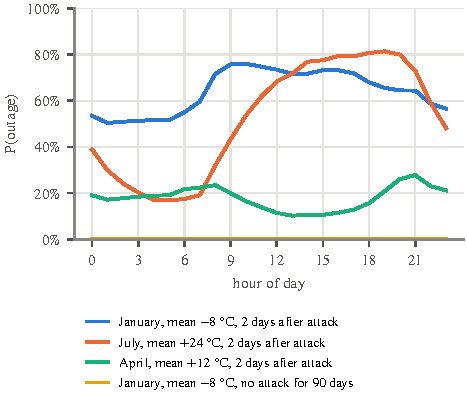
\includegraphics[width=\columnwidth]{figures/fig7_scenarios.pdf}
\caption{Predicted probability that nationwide outages are applied, by hour of a working day, in four scenarios.}
\label{fig:scen}
\end{figure}

In a frosty January two days after an attack, the risk stays between 50\% at night and 76\% at 09:00--10:00, so no part of the day is safe. On a hot July day the risk is lowest before dawn, about 17\%, and rises to 81\% at 18:00--19:00 as the heat persists and solar generation fades. In a mild April it is moderate, lowest around 13:00 at 10\% and highest at 21:00 at 28\%. In the same frosty January without attacks for 90 days, the predicted risk is practically zero.

Two reservations apply. The target is whether nationwide outages were applied in a given hour, not whether a particular consumer was disconnected. Outages rotate between queues, so the chance that a specific home or business is without power in that hour is lower. And the levels are averages over seasons, which, as Section~6 showed, do not transfer from one season to another. The scenarios are useful for comparing hours and conditions with each other: the shape of the curves is more reliable than their level.

\FloatBarrier
\section{Limitations}
The study has several limitations. First, both the outage and the strike datasets include only large-scale events, so local outages and local strikes are not modelled, and the first wave is observed only from January 2023. Second, round-the-clock days contain 70\% of outage hours, so the hourly target mostly reflects differences between days and seasons, and the number of independent episodes is small. Third, the number of hits is approximated as weapons fired minus weapons shot down, the register gives no time of day, and data on damaged facilities are not available. Fourth, the weather in Kyiv is used as a proxy for the whole country, and it is observed weather, not a forecast. Fifth, the model does not include the state of repairs, import capacity, fuel stocks and planned maintenance of nuclear units, which are not available as open hourly data. These factors probably explain why the same attacks and the same weather led to outages in one season and not in another, and why the predicted probabilities do not transfer between seasons. Finally, hourly and daily observations are dependent, so p-values and bootstrap intervals should be treated as indicative, and predictions for very hot hours above 30\,\textdegree C are uncertain because such hours are rare.

\section{Conclusion}
Using three open datasets, we built an hourly picture of planned power outages in Ukraine from 2023 to 2026. Massive attacks on energy infrastructure are a precondition for nationwide outages: without an attack in the previous 30 days outages almost never happened, even in hard frost, and they never happened later than 60 days after an attack. Attacks are not a sufficient condition: in 2025 and in spring 2026, series of attacks caused no outages. Weather amplifies outages after attacks, most clearly in summer heat, but it does not decide them: the same frost after attacks meant no outages in early 2025 and round-the-clock outages in early 2026. What decides is the state of the power system, which open data do not describe. Solar radiation is associated with lower risk once temperature is taken into account, also when measured against its seasonal norm.

A simple logistic regression with weather--attack interactions ranks hours by risk better on average than gradient boosting, and only slightly better than a baseline with attack history alone. Its probabilities are not reliable as absolute values, so it is suited to comparing conditions and hours, not to forecasting the level of outages in a new season.

Future work could add regional outage schedules, the number of disconnected queues as a measure of intensity, data on damaged facilities and import capacity, and a forecast setting that uses weather predictions instead of observed weather.

\section*{Data and Code Availability}
All datasets used in this study are publicly available from the sources listed in Table~\ref{tab:data}; raw data are not redistributed. The cleaning and analysis code is provided as two Jupyter notebooks and a script in the accompanying GitHub repository, \url{https://github.com/dkrainii/ukraine-power-outages-analysis}, together with instructions for downloading the raw data.

\renewcommand{\refname}{REFERENCES}
\renewcommand{\section}[2]{\vspace{0.6ex}\noindent{\normalsize\bfseries #2}\par\vspace{0.3ex}}
\small
\begin{thebibliography}{99}\setlength{\itemsep}{1pt}
\bibitem{breiman} L.~Breiman. Random forests. \emph{Machine Learning}, 45(1):5--32, 2001.
\bibitem{crs} Congressional Research Service. Attacks on Ukraine's electric grid: Insights for U.S.\ infrastructure security and resilience. Report R48067, May 2024.
\bibitem{dixiout} DiXi Group. Energy Map: Information on the application of electricity consumption restriction measures. Dataset, \url{https://energy-map.info}, accessed November 2026.
\bibitem{dixistr} DiXi Group. Energy Map: Information on massive strikes on the critical infrastructure of Ukraine. Dataset, \url{https://energy-map.info}, accessed November 2026.
\bibitem{dixitrade} DiXi Group. Energy Map: Hourly import and export of electricity. Dataset, \url{https://energy-map.info}, accessed November 2026.
\bibitem{friedman} J.~H.~Friedman. Greedy function approximation: A gradient boosting machine. \emph{Annals of Statistics}, 29(5):1189--1232, 2001.
\bibitem{han} S.-R.~Han, S.~D.~Guikema, S.~M.~Quiring, K.-H.~Lee, D.~Rosowsky, and R.~A.~Davidson. Estimating the spatial distribution of power outages during hurricanes in the Gulf coast region. \emph{Reliability Engineering \& System Safety}, 94(2):199--210, 2009.
\bibitem{era5} H.~Hersbach et~al. The ERA5 global reanalysis. \emph{Quarterly Journal of the Royal Meteorological Society}, 146(730):1999--2049, 2020.
\bibitem{iea} International Energy Agency. \emph{Ukraine's Energy Security and the Coming Winter}. IEA, Paris, 2024.
\bibitem{lightgbm} G.~Ke, Q.~Meng, T.~Finley, T.~Wang, W.~Chen, W.~Ma, Q.~Ye, and T.-Y.~Liu. LightGBM: A highly efficient gradient boosting decision tree. In \emph{Advances in Neural Information Processing Systems 30}, pages 3146--3154, 2017.
\bibitem{mann} H.~B.~Mann and D.~R.~Whitney. On a test of whether one of two random variables is stochastically larger than the other. \emph{Annals of Mathematical Statistics}, 18(1):50--60, 1947.
\bibitem{nateghi} R.~Nateghi, S.~D.~Guikema, and S.~M.~Quiring. Comparison and validation of statistical methods for predicting power outage durations in the event of hurricanes. \emph{Risk Analysis}, 31(12):1897--1906, 2011.
\bibitem{sklearn} F.~Pedregosa et~al. Scikit-learn: Machine learning in Python. \emph{Journal of Machine Learning Research}, 12:2825--2830, 2011.
\bibitem{sailor} D.~J.~Sailor and J.~R.~Mu\~noz. Sensitivity of electricity and natural gas consumption to climate in the U.S.A.: Methodology and results for eight states. \emph{Energy}, 22(10):987--998, 1997.
\bibitem{valor} E.~Valor, V.~Meneu, and V.~Caselles. Daily air temperature and electricity load in Spain. \emph{Journal of Applied Meteorology}, 40(8):1413--1421, 2001.
\bibitem{scipy} P.~Virtanen et~al. SciPy 1.0: Fundamental algorithms for scientific computing in Python. \emph{Nature Methods}, 17:261--272, 2020.
\bibitem{openmeteo} P.~Zippenfenig. Open-Meteo.com Weather API [Computer software]. Zenodo, 2023. \url{https://doi.org/10.5281/zenodo.7970649}.
\end{thebibliography}

\end{document}
